\documentclass{../../../oss-apphys}
\usepackage{bm}

\begin{document}
\genheader

\gentitle{1}{KINEMATICS}

\genmultidirections

\gengravity

\raggedcolumns
\begin{multicols}{2}

  \textbf{Questions 1-2}
  
  A ball of mass \SI{.5}{\kilo\gram} is launched horizontally from the top of a
  cliff \SI{80}{m} high with a speed of \SI{20}{m/s} at time $t=0$.
  \begin{center}
    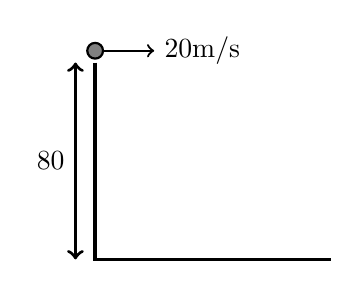
\begin{tikzpicture}[scale=.5]
      \draw[very thick](0,5)--(0,0)--(6,0);
      \draw[<->,very thick](-.5,0)--(-.5,5) node[midway,left]{\SI{80}{\metre}};
      \draw[thick,->](0,5.3)--(1.5,5.3) node[pos=1,right]{\SI{20}{m/s}};
      \draw[thick,fill=gray](0,5.3) circle(.2);
    \end{tikzpicture}
  \end{center}
  \begin{enumerate}[leftmargin=18pt]
  \item The horizontal distance $x$ traveled by the ball before striking the
    ground is
    \begin{enumerate}[noitemsep,topsep=0pt,leftmargin=18pt,label=(\Alph*)]
    \item\SI{20 }{\metre}
    \item\SI{40 }{\metre}
    \item\SI{80 }{\metre} 
    \item\SI{160}{\metre}
    \item\SI{320}{\metre}
    \end{enumerate}
  %\item Which of the following graphs best represents the vertical speed $v_y$
  %  of the ball from $t=0$ until just before the ball strikes the ground?

  \item The speed of the ball just before striking the ground is
    \begin{enumerate}[noitemsep,topsep=0pt,leftmargin=18pt,label=(\Alph*)]
    \item\SI{4 }{\metre\per\second}
    \item\SI{14}{\metre\per\second}
    \item\SI{20}{\metre\per\second}
    \item\SI{44}{\metre\per\second}
    \item\SI{64}{\metre\per\second}
    \end{enumerate}

  \item A space explorer throws a tool downward on a planet with an initial
    velocity of \SI{2.0}{m/s} from a height of \SI{6}{m} above the surface. The
    tool strikes the surface in a time of \SI{2}{\second}. The acceleration due
    to gravity on the planet is
    \begin{enumerate}[noitemsep,topsep=0pt,leftmargin=18pt,label=(\Alph*)]
    \item\SI{1 }{\metre\per\second^2}
    \item\SI{2 }{\metre\per\second^2}
    \item\SI{3 }{\metre\per\second^2}
    \item\SI{4 }{\metre\per\second^2}
    \item\SI{10}{\metre\per\second^2}
    \end{enumerate}
  \end{enumerate}
  \columnbreak

  \textbf{Questions \ref{q:sprinter1}--\ref{q:sprinter2}}
  
  A sprinter starting from rest runs a $100$-meter race on a straight track. The
  sprinter covers the first $10$ meters with a constant acceleration in $2$
  seconds. The sprinter runs the remaining \SI{90}{m} with the same velocity he
  had at the end of \SI{2}{\second}.

  \begin{enumerate}[resume,leftmargin=18pt]
  \item The sprinter's velocity at the end of the first \SI{2}{\second} is
    \begin{enumerate}[noitemsep,topsep=0pt,leftmargin=18pt,label=(\Alph*)]
    \item\SI{5 }{\metre\per\second}
    \item\SI{10}{\metre\per\second}
    \item\SI{20}{\metre\per\second}
    \item\SI{40}{\metre\per\second}
    \item\SI{60}{\metre\per\second}
    \end{enumerate}
    \label{q:sprinter1}

  \item The total time it takes for the sprinter to run the full \SI{100}{m} is
    \begin{enumerate}[noitemsep,topsep=0pt,leftmargin=18pt,label=(\Alph*)]
    \item\SI{2 }{\second}
    \item\SI{9 }{\second}
    \item\SI{10}{\second}
    \item\SI{11}{\second}
    \item\SI{12}{\second}
    \end{enumerate}
    \label{q:sprinter2}
    
  \item A block of mass \SI{2}{\kilo\gram} is attached to a string that is
    wrapped around a pulley of negligible mass and allowed to descend from rest
    a vertical distance of \SI{1.2}{\metre} in a time of \SI{1.5}{\second}. The
    acceleration of the block is most nearly
    \begin{center}
      \vspace{-.2in}
      \pic{.15}{block-pulley.png}
    \end{center}
    \begin{enumerate}[noitemsep,topsep=0pt,leftmargin=18pt,label=(\Alph*)]
    \item\SI{0.2}{\metre\per\second^2}
    \item\SI{.6}{\metre\per\second^2}
    \item\SI{1.1}{\metre\per\second^2}
    \item\SI{1.4}{\metre\per\second^2}
    \item\SI{1.5}{\metre\per\second^2}
    \end{enumerate}

%  \item A helicopter raises a package with an upward constant speed of
%    \SI{3}{m/s}. The rope suddenly breaks when the package is $8$ meters above
%    the ground. Neglecting air resistance, calculate the speed at which the
%    package strikes the ground.
%    \begin{enumerate}[noitemsep,topsep=0pt,leftmargin=18pt,label=(\Alph*)]
%    \item\SI{13 }{\metre\per\second}
%    \item\SI{26 }{\metre\per\second}
%    \item\SI{84 }{\metre\per\second}
%    \item\SI{169}{\metre\per\second}
%    \item\SI{202}{\metre\per\second}
%    \end{enumerate}
    
  \item A ball is attached to a string of length \SI{.8}{\metre} and is swung
    in a vertical circle. The bottom of the circle is \SI{.2}{\metre} above the
    floor. If the string breaks at the top of the circle when the speed of the
    ball is \SI{5}{m/s}, the horizontal distance the ball travels before
    striking the floor is
    \begin{center}
      \vspace{-.2in}
      \pic{.15}{ball-string.png}
    \end{center}
    \begin{enumerate}[noitemsep,topsep=0pt,leftmargin=18pt,label=(\Alph*)]
    \item\SI{.8 }{\metre}
    \item\SI{2.3 }{\metre}
    \item\SI{3.0 }{\metre}
    \item\SI{5.0 }{\metre}
    \item\SI{13.2}{\metre}
    \end{enumerate}
    
  \item A golf ball is hit from level ground and has a horizontal range of
    \SI{100}{m}. The ball leaves the golf club at an angle of \ang{60} to the
    level ground. At what other angle(s) can the ball be struck at the same
    initial velocity and still have a range of \SI{100}{m}?
    \begin{center}
      \vspace{-.2in}
      \pic{.25}{golf-ball.png}
    \end{center}
    \begin{enumerate}[noitemsep,topsep=0pt,leftmargin=18pt,label=(\Alph*)]
    \item\ang{30}
    \item\ang{20} and \ang{80}
    \item\ang{10} and \ang{120}
    \item\ang{45} and \ang{135}
    \item There is no other angle other than \ang{60} in which the ball will
      have a range of \SI{100}{m}.
    \end{enumerate}
    
  \item A small airplane can fly at \SI{200}{km/h} with no wind. The pilot of
    the plane would like to fly to a destination \SI{100}{km} due north of his
    present position, but there is a crosswind of \SI{50}{km/h} east. How much
    time is required for the plane to fly north to its destination?
    \begin{enumerate}[noitemsep,topsep=0pt,leftmargin=18pt,label=(\Alph*)]
    \item less than \SI{1/2}{\hour}
    \item \SI{1/2}{\hour}
    \item more than \SI{1/2}{\hour}
    \item \SI{1}{\hour}
    \item more than \SI{1}{\hour}
    \end{enumerate}
    
  \end{enumerate}
  \columnbreak
  
  \textbf{Questions \ref{q:particle1}--\ref{q:particle2}}

  A particle moves on a horizontal surface with a constant acceleration of
  \SI{6}{m/s^2} in the $x$-direction and \SI{4}{m/s^2} in the $y$-direction. The
  initial velocity of the particle is \SI{3}{m/s} in the $x$-direction.
  
  \begin{enumerate}[resume,leftmargin=18pt]
  \item The speed of the particle after \SI{4}{\second} is
    \begin{enumerate}[noitemsep,topsep=0pt,leftmargin=18pt,label=(\Alph*)]
    \item\SI{16 }{\metre\per\second}
    \item\SI{27 }{\metre\per\second}
    \item\SI{31 }{\metre\per\second}
    \item\SI{44 }{\metre\per\second}
    \item\SI{985}{\metre\per\second}
    \end{enumerate}
    \label{q:particle1}
    
  \item The displacement of the particle from its initial position is
    \begin{enumerate}[noitemsep,topsep=0pt,leftmargin=18pt,label=(\Alph*)]
    \item\SI{16}{\metre}
    \item\SI{32}{\metre}
    \item\SI{60}{\metre}
    \item\SI{68}{\metre}
    \item\SI{92}{\metre}
    \end{enumerate}
    \label{q:particle2}
    
%  \textf{Questions 14-15}
%
%  The graph shown represents the motion of a cart rolling along a horizontal
%track.
%14. The time(s) at which the object is at rest is
%(A) zero
%(B) 8 s and 36 s
%(C) 18 s and 40 s
%(D) 24 s and 34 s
%(E) 40 s and 50 s
%15. The time(s) at which the cart changes direction is
%(A) zero
%(B) 8 s and 36 s
%(C) 18 s and 40 s
%(D) 24 s and 34 s
  %(E) 40 s and 50 s
    
  \item A rubber ball is dropped from rest onto a plane angled at \ang{30} to
    the horizontal floor and bounces off the plane with a horizontal speed
    $v_o$. The ball lands on the plane a distance $D$ along the plane, as shown
    below. In terms of $v_o$, $D$, and $g$, the speed of the ball just before
    striking the plane is
    \begin{center}
      \pic{.25}{bounce.png}
    \end{center}
    \begin{enumerate}[noitemsep,topsep=0pt,leftmargin=18pt,label=(\Alph*)]
    \item $v_o$
    \item $\displaystyle\left(v_o^2+2D\sin\theta g\right)^\frac{1}{2}$
    \item $\displaystyle\left(v_o+\frac{D\sin\theta}{g}\right)^\frac{1}{2}$
    \item $\displaystyle\left(v_o^2+\frac{D\sin\theta}{g}\right)^\frac{1}{2}$
    \item $\displaystyle\left(2D\sin\theta g\right)^\frac{1}{2}$
    \end{enumerate}
    \columnbreak
    
%\item Which of the following best represents the graph of velocity vs.\ time
%  from $t = 0$ until the filters reach terminal velocity?
    %  \begin{enumerate}[noitemsep,topsep=0pt,leftmargin=18pt,label=(\Alph*)]
    \columnbreak
    
  \item A small ball is launched with a speed of \SI{8}{m/s} at an angle of
    \ang{30} from the horizontal. A cup is hung so that it is in position to
    catch the ball when it reaches its maximum height. How far above the floor
    should the cup be hung to catch the ball?
    
    \pic{.35}{cup.png}

    \begin{enumerate}[noitemsep,topsep=0pt,leftmargin=18pt,label=(\Alph*)]
    \item\SI{2.4}{\metre}
    \item\SI{1.6}{\metre}
    \item\SI{1.0}{\metre}
    \item\SI{.8}{\metre}
    \item\SI{.4}{\metre}
    \end{enumerate}
  \end{enumerate}
  
  \textbf{Questions \ref{q:graph1}--\ref{q:graph2}}

  The graph shown below represents the velocity vs.\ time graphs for two cars,
  $P$ and $Q$. Car $P$ begins with a speed $v_P$, and Car $Q$ begins with a
  speed $v_Q$ which is twice the velocity of Car $P$, that is, $v_Q=2v_P$.
  \begin{center}
    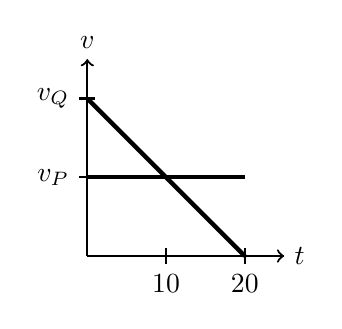
\begin{tikzpicture}[scale=.5]
      \draw[thick,->](0,0)--(5,0) node[pos=1,right]{$t$};
      \draw[thick,->](0,0)--(0,5) node[pos=1,above]{$v$};
      \draw[ultra thick](0,4)--(4,0);
      \draw[ultra thick](0,2)--(4,2);
      \draw[thick](2,.2)--(2,-.2) node[pos=1,below]{10};
      \draw[thick](4,.2)--(4,-.2) node[pos=1,below]{20};
      \draw[thick](.2,4)--(-.2,4) node[pos=1,left]{$v_Q$};
      \draw[thick](.2,2)--(-.2,2) node[pos=1,left]{$v_P$};
      \end{tikzpicture}
  \end{center}
  \begin{enumerate}[resume,leftmargin=18pt]
  \item Which of the following is true at a time of \SI{10}{\second}?
    \begin{enumerate}[noitemsep,topsep=0pt,leftmargin=18pt,label=(\Alph*)]
    \item The cars occupy the same position.
    \item Car $P$ is at rest.
    \item $v_Q>v_P$
    \item $v_P>v_Q$
    \item Car $Q$ is ahead of Car $P$.
    \end{enumerate}
    \label{q:graph1}
    
  \item Which of the following is true at a time of \SI{20}{\second}?
    \begin{enumerate}[noitemsep,topsep=0pt,leftmargin=18pt,label=(\Alph*)]
    \item The cars occupy the same position.
    \item Car $P$ is at rest.
    \item $v_Q>v_P$
    \item $a_P=a_Q$
    \item Car $P$ is ahead of Car $Q$.
    \end{enumerate}
    \label{q:graph2}
    
  \item The velocity vs.\ time graph below represents the motion of a bicycle
    rider. The displacement of the rider between $0$ and \SI{4}{\hour} is
    \begin{center}
      \pic{.25}{bikerider.png}
    \end{center}
    \begin{enumerate}[noitemsep,topsep=0pt,leftmargin=18pt,label=(\Alph*)]
    \item +\SI{10}{\kilo\metre}
    \item +\SI{20}{\kilo\metre}
    \item +\SI{30}{\kilo\metre}
    \item +\SI{40}{\kilo\metre}
    \item -\SI{10}{\kilo\metre}
    \end{enumerate}
    
  \item A car is initially moving with a positive velocity of \SI{20}{m/s} when
    it passes the origin at time $t=0$. The car continues to move at
    \SI{20}{\metre\per\second} between $t=0$ and $t=\SI{2}{\second}$. At
    $t=\SI{2}{\second}$, the driver presses the brake, giving the car an
    acceleration of \SI{-4}{\metre\per\second^2}. The displacement of the car
    at $t=\SI{6}{\second}$ is
    \begin{enumerate}[noitemsep,topsep=0pt,leftmargin=18pt,label=(\Alph*)]
    \item\SI{40}{\metre}
    \item\SI{32}{\metre}
    \item\SI{48}{\metre}
    \item\SI{64}{\metre}
    \item\SI{88}{\metre}
    \end{enumerate}

  \item A ball is dropped from rest from the top of a cliff $80$ meters high. At
    the same time, a rock is thrown horizontally from the top of the same
    cliff. The rock and ball hit the level ground below a distance of
    \SI{40}{\metre} apart. The horizontal velocity of the rock that was thrown
    was most nearly
    \begin{center}
      \vspace{-.15in}\pic{.25}{ball-cliff.png}
    \end{center}
    \begin{enumerate}[noitemsep,topsep=0pt,leftmargin=18pt,label=(\Alph*)]
    \item\SI{5}{\metre\per\second}
    \item\SI{10}{\metre\per\second}
    \item\SI{20}{\metre\per\second}
    \item\SI{40}{\metre\per\second}
    \item\SI{80}{\metre\per\second}
    \end{enumerate}
    \columnbreak
    
  \item Which of the following pairs of graphs could show the position vs.\
    time and velocity vs.\ time graphs for the acceleration vs. time graph
    shown above? Assume $v=0$ and $x=0$ at $t=0$.
    \begin{center}
      \begin{tikzpicture}[scale=.5]
        \draw[thick,->](0,0)--(8,0) node[pos=1,right]{$t$};
        \draw[thick,->](0,-3)--(0,3) node[pos=1,above]{$a$};
        \draw[ultra thick](0,2)--(2,2);
        \draw[ultra thick](2,0)--(4,0);
        \draw[ultra thick](4,-2)--(6,-2);
        \draw[ultra thick](6,0)--(8,0);
        \draw[thick,dashed](2,2)--(2,0);
        \draw[thick,dashed](4,0)--(4,-2);
        \draw[thick,dashed](6,0)--(6,-2);
      \end{tikzpicture}
    \end{center}
    \pic{.48}{xt-vt.png}

  \item A stone is dropped near the surface of Mars and falls with an
    acceleration of \SI{3.8}{m/s^2}. This means that the
    \begin{enumerate}[noitemsep,topsep=0pt,leftmargin=18pt,label=(\Alph*)]
    \item distance the stone falls increases 3.8 meters for each second of
      fall
    \item derivative of the distance fallen with respect to time is
      \SI{3.8}{m/s}
    \item derivative of the velocity with respect to time is \SI{3.8}{m/s^2}
    \item velocity is constant at \SI{3.8}{m/s}
    \item derivative of the acceleration is \SI{3.8}{m/s^2}
    \end{enumerate}    
    \columnbreak
    
  \item Two velocity vectors $v_1$ and $v_2$ each have a magnitude of 10 m/s.
    Graph 1 shows the velocity $v_1$ at $t =\SI{0}{\second}$, and then the same
    object has a velocity $v_2$ at $t=\SI{2}{\second}$, shown in Graph 2. Which
    of the following vectors best represents the average acceleration vector
    that causes the object's velocity to change from $v_1$ to $v_2$ ?
    \begin{center}
      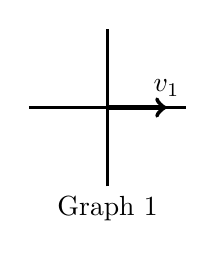
\begin{tikzpicture}[scale=.5]
        \draw[thick](-2,0)--(2,0);
        \draw[thick](0,-2)--(0,2) node[pos=0,below]{Graph 1};
        \draw[ultra thick,->](0,0)--(1.5,0) node[pos=1,above]{$v_1$};
      \end{tikzpicture}
      \hspace{.2in}
      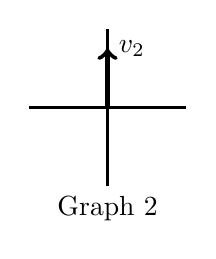
\begin{tikzpicture}[scale=.5]
        \draw[thick](-2,0)--(2,0);
        \draw[thick](0,-2)--(0,2) node[pos=0,below]{Graph 2};
        \draw[ultra thick,->](0,0)--(0,1.5) node[pos=1,right]{$v_2$};
      \end{tikzpicture}
    \end{center}
    \begin{enumerate}[noitemsep,topsep=0pt,leftmargin=18pt,label=(\Alph*)]
    \item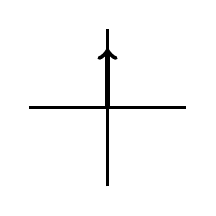
\begin{tikzpicture}[scale=.5]
      \draw[thick](-2,0)--(2,0);
      \draw[thick](0,-2)--(0,2);
        \draw[ultra thick,->](0,0)--(0,1.5);
    \end{tikzpicture}
    \item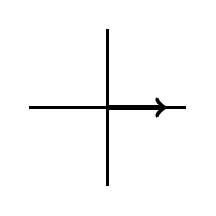
\begin{tikzpicture}[scale=.5]
      \draw[thick](-2,0)--(2,0);
      \draw[thick](0,-2)--(0,2);
      \draw[ultra thick,->](0,0)--(1.5,0);
    \end{tikzpicture}
    \item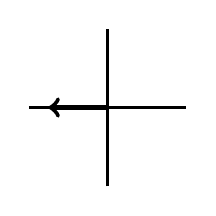
\begin{tikzpicture}[scale=.5]
        \draw[thick](-2,0)--(2,0);
        \draw[thick](0,-2)--(0,2);
        \draw[ultra thick,->](0,0)--(-1.5,0);
    \end{tikzpicture}
    \item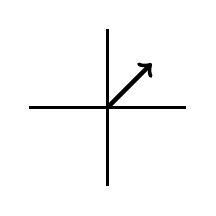
\begin{tikzpicture}[scale=.5]
      \draw[thick](-2,0)--(2,0);
      \draw[thick](0,-2)--(0,2);
        \draw[ultra thick,->](0,0)--(1.12,1.12);
    \end{tikzpicture}
    \item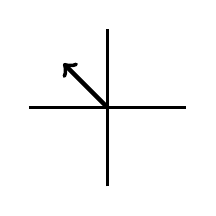
\begin{tikzpicture}[scale=.5]
      \draw[thick](-2,0)--(2,0);
      \draw[thick](0,-2)--(0,2);
        \draw[ultra thick,->](0,0)--(-1.12,1.12);
    \end{tikzpicture}
    \end{enumerate}
    \columnbreak
    
  \item A \SI{600}{\kilo\gram} car accelerates uniformly from rest. After
    \SI{4}{\second}, it reaches a speed of \SI{24}{m/s}. During the
    \SI{4}{\second}, the car has traveled a distance of
    \begin{enumerate}[noitemsep,topsep=0pt,leftmargin=18pt,label=(\Alph*)]
    \item\SI{12}{\metre}
    \item\SI{24}{\metre}
    \item\SI{36}{\metre}
    \item\SI{48}{\metre}
    \item\SI{96}{\metre}
    \end{enumerate}

  item A toy dart gun fires a dart at an angle of \ang{45} to the horizontal
    and the dart reaches a maximum height of $1$ meter. If the dart were fired
    straight up into the air along the vertical, the dart would reach a height
    of
    \begin{enumerate}[noitemsep,topsep=0pt,leftmargin=18pt,label=(\Alph*)]
    \item\SI{1}{\metre}
    \item\SI{2}{\metre}
    \item\SI{3}{\metre}
    \item\SI{4}{\metre}
    \item\SI{5}{\metre}
    \end{enumerate}
    
  \item A passenger on a train moving horizontally at a constant speed relative
    to the ground drops a ball from his window. A stationary observer on the
    ground sees the ball falling with a speed $v_1$ at an angle to the vertical
    at the instant it is dropped from the train window, but the ball appears to
    be falling vertically with a speed $v_2$ at the same instant as viewed by
    the train passenger. What is the speed (magnitude of velocity) of the train
    relative to the ground after the ball is dropped? Neglect air resistance.
    \begin{enumerate}[noitemsep,topsep=0pt,leftmargin=18pt,label=(\Alph*)]
    \item $ v_1 + v_2$
    \item $ v_1 - v_2$
    \item $ v_1^2 + v_2^2$
    \item $ v_1^2 - v_2^2$
    \item $\sqrt{v_1^2 - v_2^2}$
    \end{enumerate}
      
  \item A ball is hit straight up into the air with an upward positive
    velocity. Wich of the following describes the velocity and acceleration
    of the ball at the instant it reaches the top of its flight?
    \begin{tabular}{lcc}
      & Velocity & Acceleration\\ \hline
      (A) & $0$ & $0$\\
      (B) & $0$ & $g$\\
      (C) & $2v_0$ & $g$\\
      (D) & $\frac{1}{2}v_0$ & $0$\\
      (E) & $0$ & $\frac{1}{2}g$
    \end{tabular}    
    
  \item A student jumps off a cliff with an initial horizontal velocity $v$ and
    lands in a lake below at a distance of $x$ from the base of the cliff. In
    terms of his initial velocity $v$, how fast would he have had to jump to
    land a distance $2x$ from the base of the cliff?
    \begin{center}
      \begin{tikzpicture}[scale=.5]
        \draw[thick](0,4)--(0,0)--(6,0);
        \draw[thick,->](0,4.2)--(1,4.2) node[pos=1,right]{$v$};
        \draw[fill=gray,thick] (0,4.2) circle(.1);
        \draw[thick](2,.2)--(2,-.2) node[pos=1,below]{$x$};
        \draw[thick](4,.2)--(4,-.2) node[pos=1,below]{$2x$};
      \end{tikzpicture}
    \end{center}
    \begin{enumerate}[noitemsep,topsep=0pt,leftmargin=18pt,label=(\Alph*)]
    \item $\sqrt{2v}$
    \item $2v$
    \item $4v$
    \item $8v$
    \item $16v$
    \end{enumerate}
    
  \item An astronaut drops a hammer on a moon with no atmosphere. The hammer
    falls a distance of $2$ meters in the first second. What is the
    acceleration due to gravity on this moon?
    \begin{enumerate}[noitemsep,topsep=0pt,leftmargin=18pt,label=(\Alph*)]
    \item\SI{1}{\metre\per\second^2}
    \item\SI{2}{\metre\per\second^2}
    \item\SI{3}{\metre\per\second^2}
    \item\SI{4}{\metre\per\second^2}
    \item\SI{8}{\metre\per\second^2}
    \end{enumerate}

  \item A car travels \SI{300}{\metre} in \SI{60}{\second}, then travels
    \SI{200}{\metre} in \SI{30}{\second}. The average speed of the car is
    \begin{enumerate}[noitemsep,topsep=0pt,leftmargin=18pt,label=(\Alph*)]
    \item\SI{5.6}{\metre\per\second}
    \item\SI{5.0}{\metre\per\second}
    \item\SI{3.0}{\metre\per\second}
    \item\SI{2.3}{\metre\per\second}
    \item\SI{12.}{\metre\per\second}
    \end{enumerate}
    \columnbreak
    
  \item The motion of an object is represented by the acceleration vs.\ time
    graph below. The object begins from rest. Which of the following statements
    is true about the motion of the object?
    \begin{center}
      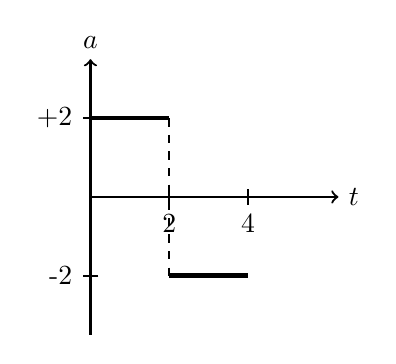
\begin{tikzpicture}[scale=.5]
        \draw[thick,->](0,0)--(6.3,0) node[pos=1,right]{$t$};
        \draw[thick,->](0,-3.5)--(0,3.5) node[pos=1,above]{$a$};
        \draw[ultra thick](0,2)--(2,2);
        \draw[ultra thick](2,-2)--(4,-2);
        \draw[dashed,thick](2,2)--(2,-2);
        \draw[thick](2,.2)--(2,-.2) node[pos=1,below]{2};
        \draw[thick](4,.2)--(4,-.2) node[pos=1,below]{4};
        \draw[thick](.2,2)--(-.2,2) node[pos=1,left]{+2};
        \draw[thick](.2,-2)--(-.2,-2) node[pos=1,left]{-2};
      \end{tikzpicture}
    \end{center}
    \begin{enumerate}[noitemsep,topsep=0pt,leftmargin=18pt,label=(\Alph*)]
    \item The object returns to its original position.
    \item The velocity of the object is zero at a time of \SI{2}{\second}.
    \item The velocity of the object is zero at a time of \SI{4}{\second}.
    \item The displacement of the object is zero at a time of \SI{4}{\second}.
    \item The acceleration of the object is zero at a time of \SI{2}{\second}.
    \end{enumerate}
    \columnbreak
    
  \item The graph below shows the displacement as a function of time for a
    car moving in a straight line. Which of the following graphs shows the
    velocity vs.\ time graph for the same time intervals?
    \begin{center}
      \pic{.25}{xt.png}
    \end{center}
    \pic{.3}{ab.png}
    \pic{.38}{cde.png}
    
%Free ResponseThe acceleration vs. time graph shows the motion of an elevator during a 20-
%second time interval. The elevator starts from rest at time t = .
%46. Determine the instantaneous velocity of the elevator at the end of 10 s.
%47. Determine the displacement of the elevator after 5 s.
%48. On the axes below, sketch the graph that represents the velocity vs.
%time graph for the elevator for the 20-second time interval.Questions 49–5. A particle follows a parabolic path with the equation y =
%2x 2 as shown. The x-component of the particle’s velocity v x as a function of
%time t is 6, that is, the horizontal displacement is x = 6t.
%49. Determine the y-component of the particle’s velocity v y as a function
%of time.
%5. On the diagram below, sketch arrows to represent the horizontal and
%vertical components of the particle’s acceleration at point P.
   
  \end{enumerate}
\end{multicols}

\newpage
%\begin{center}
%  {\Large
%    \textbf{AP\textsuperscript{\textregistered} Physics 1 \&C: Kinematics\\
%      Student Answer Sheet for Multiple-Choice Section}
%  }
%  
%  \begin{minipage}[t]{.3\textwidth}
%  \vspace{.2in}
%  \bgroup
%  \begin{tabular}{>{\centering}m{1.3cm} >{\centering}m{1.7cm}}
%    No. & Answer
%  \end{tabular}\\
%  \def\arraystretch{1.5}
%  \begin{tabular}{|>{\centering}m{1.3cm}|>{\centering}m{1.7cm}|}
%    \hline
%    1 & \\ \hline
%    2 & \\ \hline
%    3 & \\ \hline
%    4 & \\ \hline
%    5 & \\ \hline
%    6 & \\ \hline
%    7 & \\ \hline
%    8 & \\ \hline
%    9 & \\ \hline
%    10 & \\ \hline
%    11 & \\ \hline
%    12 & \\ \hline
%    13 & \\ \hline
%    14 & \\ \hline
%    15 & \\ \hline
%    16 & \\ \hline
%    17 & \\ \hline
%    18 & \\ \hline
%    19 & \\ \hline
%    20 & \\ \hline
%    21 & \\ \hline
%    22 & \\ \hline
%    23 & \\ \hline
%    24 & \\ \hline
%    25 & \\ \hline
%  \end{tabular}
%  \egroup
%  \end{minipage}
%  \begin{minipage}[t]{.3\textwidth}
%  \vspace{.2in}
%  \bgroup
%  \begin{tabular}{>{\centering}m{1.3cm} >{\centering}m{1.7cm}}
%    No. & Answer
%  \end{tabular}\\
%  \def\arraystretch{1.5}
%  \begin{tabular}{|>{\centering}m{1.3cm}|>{\centering}m{1.7cm}|}
%    \hline
%    26 & \\ \hline
%    27 & \\ \hline
%    28 & \\ \hline
%    29 & \\ \hline
%    30 & \\ \hline
%    31 & \\ \hline
%    32 & \\ \hline
%    33 & \\ \hline
%    34 & \\ \hline
%    35 & \\ \hline
%    36 & \\ \hline
%    37 & \\ \hline
%    38 & \\ \hline
%  \end{tabular}
%  \egroup
%  \end{minipage}
%\end{center}
%\newpage

\genfreetitle{1 \& C}{KINEMATICS}{5}

\genfreedirections{10}

\begin{enumerate}[leftmargin=15pt]

%\item The acceleration vs.\ time graph shows the motion of an elevator during a
%  $20$-second time interval. The elevator starts from rest at time $t=0$. 
%  \begin{center}
%    \pic{.5}{a-t.png}
%  \end{center}
%  \begin{enumerate}[noitemsep]
%  \item Determine the instantaneous velocity of the elevator at the end of
%    \SI{10}{\second}.
%    \vspace{1in}
%  \item Determine the displacement of the elevator after \SI{5}{\second}.
%    \vspace{1in}
%  \item On the axes below, sketch the graph that represents the velocity vs.\
%    time graph for the elevator for the $20$-second time interval.
%    \begin{center}
%      \pic{.5}{v-t.png}
%    \end{center}
%    \newpage
%  \end{enumerate}
%  
%\item A particle follows a parabolic path with the equation $y=2x^2$ as shown.
%  The $x$-component of the particle's position is given by $x=3t^2$.
%  \begin{center}
%    \begin{tikzpicture}[scale=1.1]
%      \draw[very thick,->](0,0)--(5,0) node[pos=1,right]{$x$};
%      \draw[very thick,->](0,0)--(0,4) node[pos=1,above]{$y$};
%      \draw[very thick,smooth,samples=20,domain=0:4.2] plot(\x,{.2*\x*\x});
%      \draw[fill=black](3,1.8) circle(.05) node[right]{$P$};
%    \end{tikzpicture}
%  \end{center}
%  \begin{enumerate}[noitemsep]
%  \item Determine the $y$-component of the particle's velocity $v_y$ as a
%    function of time.
%  \item On the diagram above, sketch arrows to represent the horizontal and
%    vertical components of the particle's acceleration at point $P$.
%  \end{enumerate}
%
%\item Given an object whose displacement is given by $x(t)=3t^3+3t^2$, find
%  \begin{enumerate}[noitemsep,topsep=0pt]
%  \item Its average velocity between $t=\SI{2}{\s}$ and $t=\SI{5}{\s}$.
%  \item Its instantaneous velocity at $t=\SI{2}{\s}$.
%  \item Its acceleration at $t=\SI{2}{\s}$.
%  \item If its mass is \SI{2}{\kg}, find the net force on this object as a
%    function of time.
%  \end{enumerate}
%  \newpage

\item An object has a position vector given by
  $\mb{r}=30t\bm{\hat{\imath}}+(40t-5t^2)\bm{\hat{\jmath}}$. Find
%\item An object moves on a plane as
%  $\displaystyle \mb{d}(t)=2t^2\bm{\hat{\imath}}+\frac{1}{t}\bm{\hat{\jmath}}$
%  for $t\geq\SI{2}{\s}$. Find
  \begin{enumerate}[noitemsep,topsep=0pt]
  \item its intantaneous velocity and acceleration vectors as functions of time
  \item its displacement after $t=\SI{3}{\s}$.
%  \item its velocity and speed at $t=\SI{3}{\s}$.
%  \item its acceleration as a function of time and the magnitude of the
%    acceleration.
  \end{enumerate}
  \vspace{2in}

\item The position $x$ of an object is described with respect to time $t$ by
  the following equation: $x=2t^3-15t^2+36t-8$. Answer the following questions.
  \begin{enumerate}[noitemsep,topsep=0pt]
  \item Find its displacement between $t=\num{3}$ and \SI{5}{\second}.
  \item Write out an expression for the velocity of the object with respect to
    time.
  \item Write out an expression for the acceleration of the object with respect
    to time.
  \item At what point(s) in time is the velocity of the object zero?
    \label{partd}
  \item At each of those points (from \ref{partd} above), is the acceleration
    positive, negative, or zero?
  \item During what intervals of time is the velocity of the object positive?
  \item During what intervals of time is the acceleration of the object
    positive?
  \item On the graph (on the next page), sketch position $x$, velocity $v$ and
    acceleration $a$ as functions of time.
  \end{enumerate}
  \newpage
  \begin{center}
    \begin{tikzpicture}[scale=.9]
      \draw[thick,->](0,-3)--(0,3) node[pos=1,above]{$x$};
      \draw[thick,->](0,0)--(10,0) node[pos=1,above]{$t$};
    \end{tikzpicture}

    \begin{tikzpicture}[scale=.9]
      \draw[thick,->](0,-3)--(0,3) node[pos=1,above]{$v$};
      \draw[thick,->](0,0)--(10,0) node[pos=1,above]{$t$};
    \end{tikzpicture}

    \begin{tikzpicture}[scale=.9]
      \draw[thick,->](0,-3)--(0,3) node[pos=1,above]{$a$};
      \draw[thick,->](0,0)--(10,0) node[pos=1,above]{$t$};
    \end{tikzpicture}
  \end{center}
  \newpage

  % Tipler Chapter 3 Question 72
\item A projectile is launched from point O at an angle of \ang{22} with an
  initial velocity of \SI{15}{\metre\per\second} up an incline plane that makes
  an angle of \ang{10} with the horizontal. The projectile hits the incline
  plane at point M.
  \begin{center}
    \pic{.35}{incline.png}
  \end{center}
  \begin{enumerate}[noitemsep,topsep=0pt]
  \item Find the time it takes for the projectile to hit the incline plane.
  \item Find the distance OM.
  \end{enumerate}
  \vspace{1.75in}
  
\item A steel ball is dropped from a point with $(x,y)$ coordinate of
  $(\SI{8}{\metre},\SI{16}{\metre})$. At the same time, another ball is launched
  from the origin with a speed of \SI{20}{\metre\per\second} at an angle of
  \ang{30}.
  \begin{enumerate}[noitemsep,topsep=0pt]
  \item Find the minimum distance of separation occur of the two balls.
  \item At what time does this separation occur?
  \item Give the coordinates of the two balls for the minimum separation.
  \end{enumerate}
  \newpage

\item A high-powered rifle shoots bullets that leave the mizzle at
  \SI{1.1e3}{\metre\per\second}. If a bullet is to hit a target
  \SI{950}{\metre} away at the level, the gun must be aimed at a point above
  the target. Neglecting air resistance, how far above the target is this
  point? 
  \vspace{2in}

\item A trail bike take off from a ramp with velocity $\mb{v}_0$ at angle
  $\theta$ to clear a ditch of width $x$ and land on the other side, which is
  elevated at a height $H$.
  \begin{center}
    \pic{.4}{trail-bike.jpg}
  \end{center}
  \begin{enumerate}[noitemsep,topsep=0pt]
  \item For a given angle $\theta$ and distance $x$, what is the upper limit
    for $H$ such that the bike has an chance of making the jump?
  \item For $H$ less than this upper limit, what is the minimum take-off speed
    $v_0$ necessary for a successful jump?
  \end{enumerate}
  Neglect the size of the trail bike, and assume that covering a horizontal
  distance $x$ and a vertical distance $H$ is sufficient to clear the ditch.
\end{enumerate}
\end{document}
